\begin{figure}
	\centering
	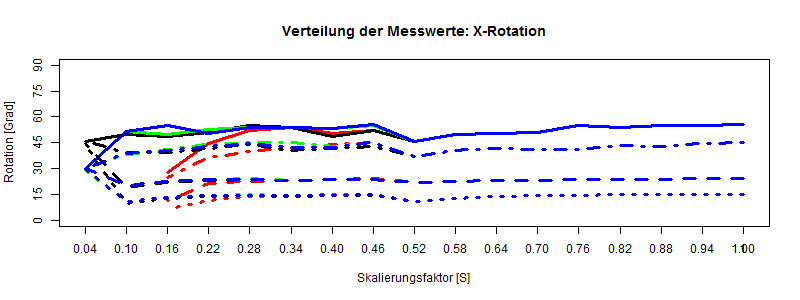
\includegraphics[width=\linewidth]{img_Skalierung/Skal_Max_RX}
	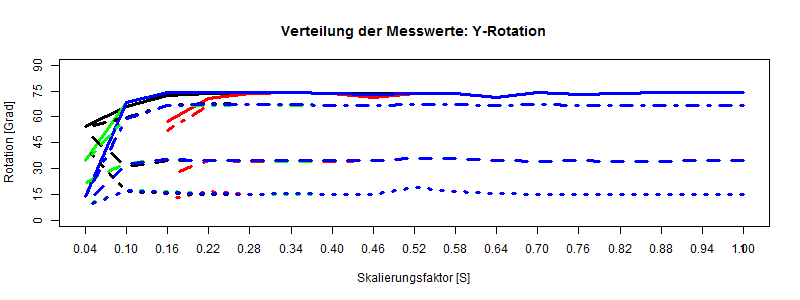
\includegraphics[width=\linewidth]{img_Skalierung/Skal_Max_RY}
	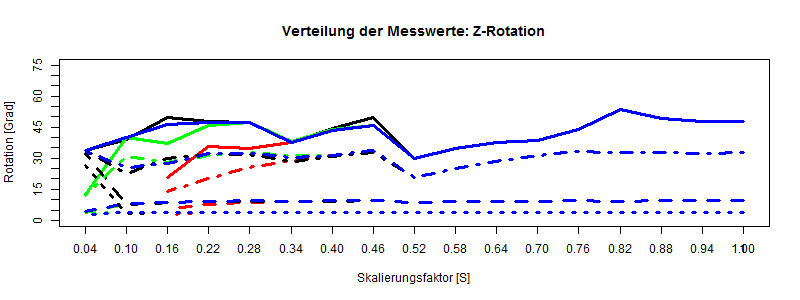
\includegraphics[width=\linewidth]{img_Skalierung/Skal_Max_RZ}
	\caption{Dargestellt ist der Bereich in denen im BIWI \cite{database_Face_Ori} ein Gesicht erkannt wurde.\\
		Bicubic (blau), Lanczos (grün), Linear (schwarz), Nearest-Neighbor (rot)\\
		Maximal erreichter Wert: \protect
\includegraphics[width=0.15\linewidth]{line/Line1}\\
		$99\%$ Quantile der Messwerte: \protect
\includegraphics[width=0.15\linewidth]{line/Line4}\\
		$80\%$ Quantile der Messwerte:\protect
\includegraphics[width=0.15\linewidth]{line/Line2}\\
		Median aus den Messwerten: \protect
\includegraphics[width=0.15\linewidth]{line/Line3}}
	\label{img_Rot_Max}
\end{figure}
\begin{landscape}
\begin{figure}
	\centering
	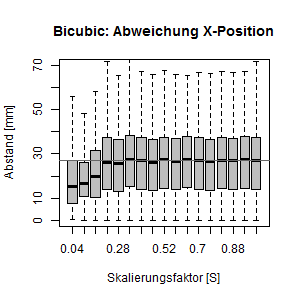
\includegraphics[width=0.245\linewidth]{img_Skalierung/CU_Tx}
	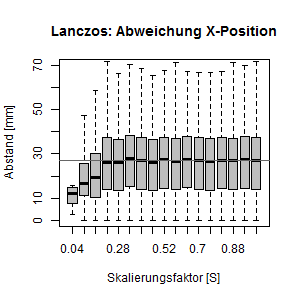
\includegraphics[width=0.245\linewidth]{img_Skalierung/LA_Tx}
	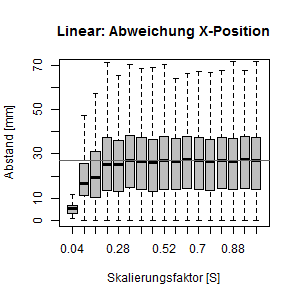
\includegraphics[width=0.245\linewidth]{img_Skalierung/LI_Tx}
	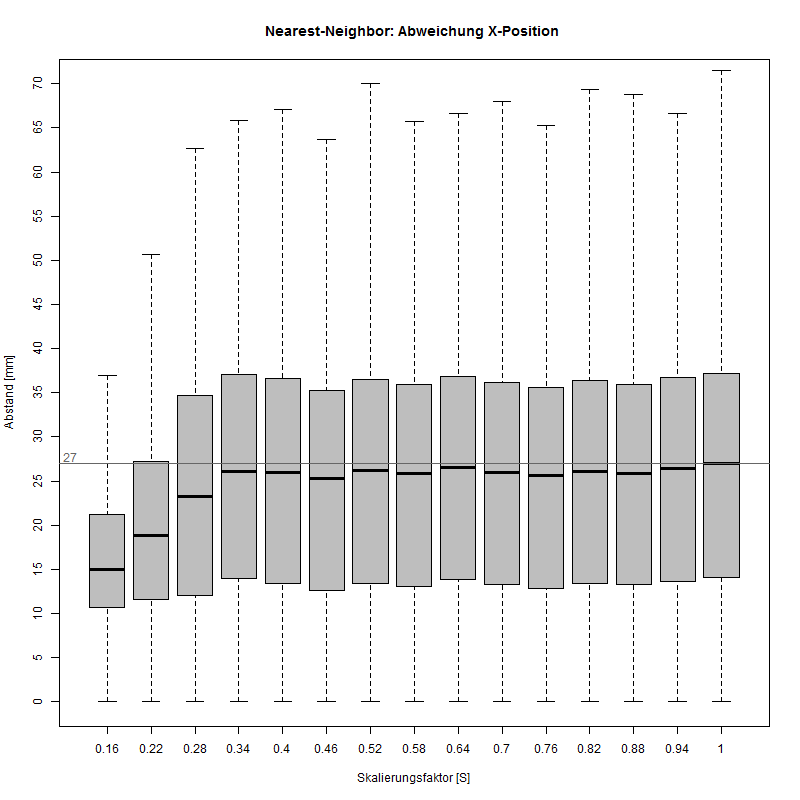
\includegraphics[width=0.245\linewidth]{img_Skalierung/NN_Tx}
	\caption{Zusammenhang zwischen der Skalierung und der Abweichung in X-Richtung in Millimeter.\\
		Von rechts nach links: Bicubic, Lanczos, Linear, Nearest-Neighbor}
	\label{img_X_Pos_Skal}
\end{figure}
\begin{figure}
	\centering
	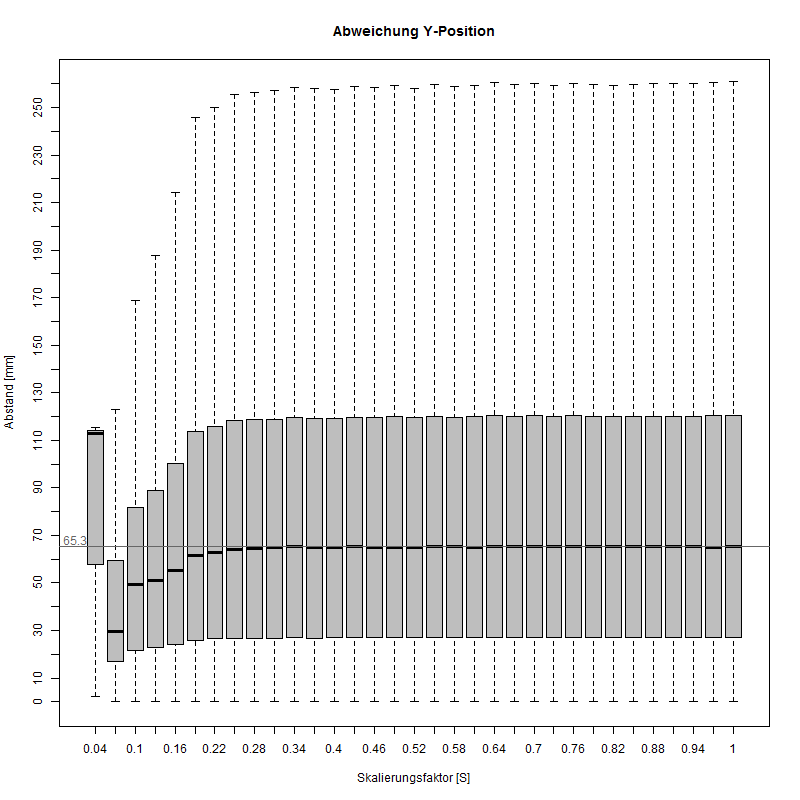
\includegraphics[width=0.245\linewidth]{img_Skalierung/CU_Ty}
	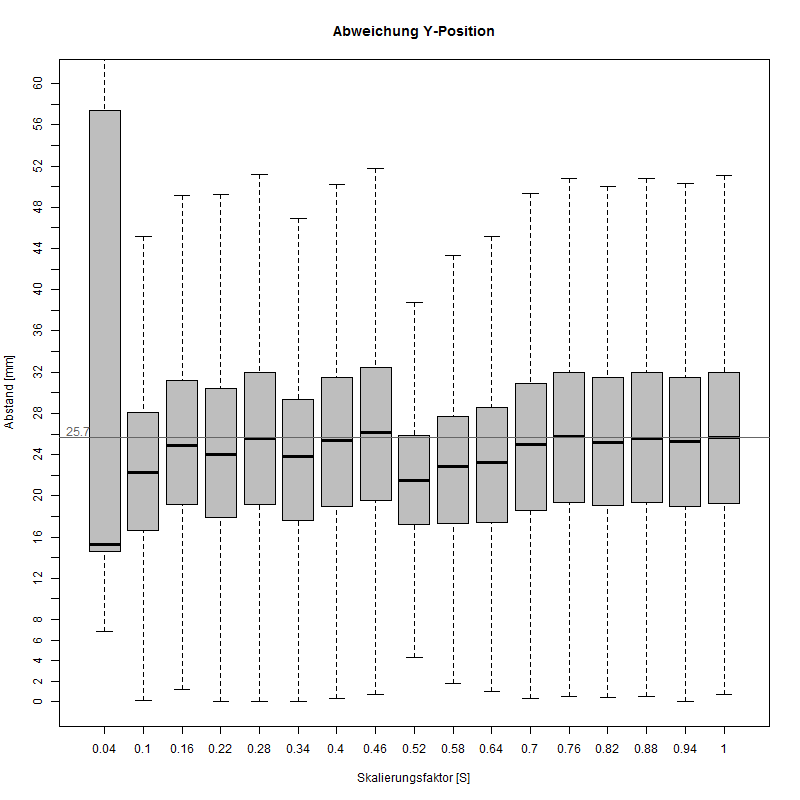
\includegraphics[width=0.245\linewidth]{img_Skalierung/LA_Ty}
	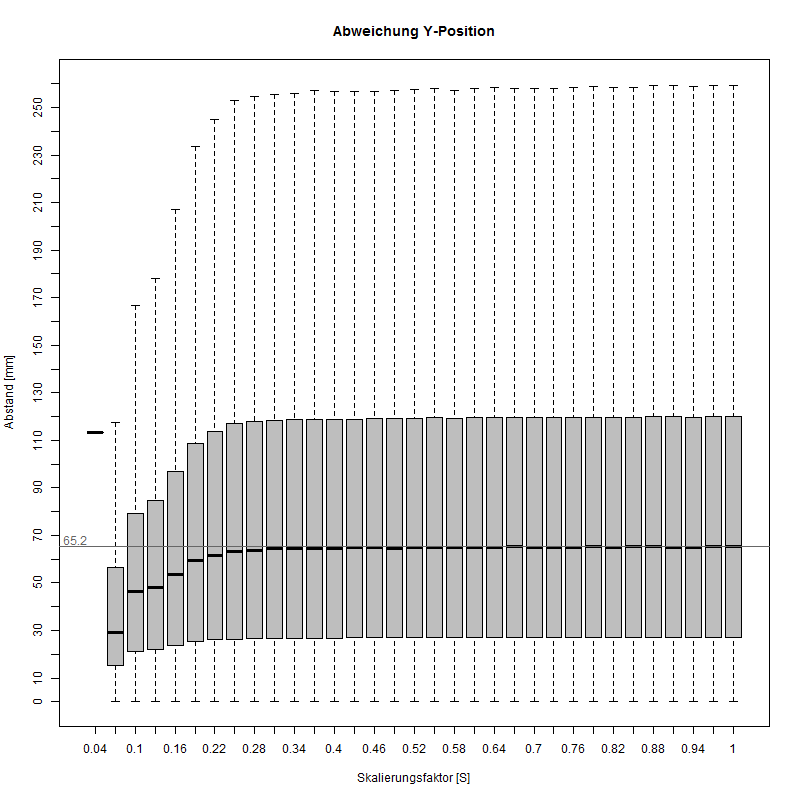
\includegraphics[width=0.245\linewidth]{img_Skalierung/LI_Ty}
	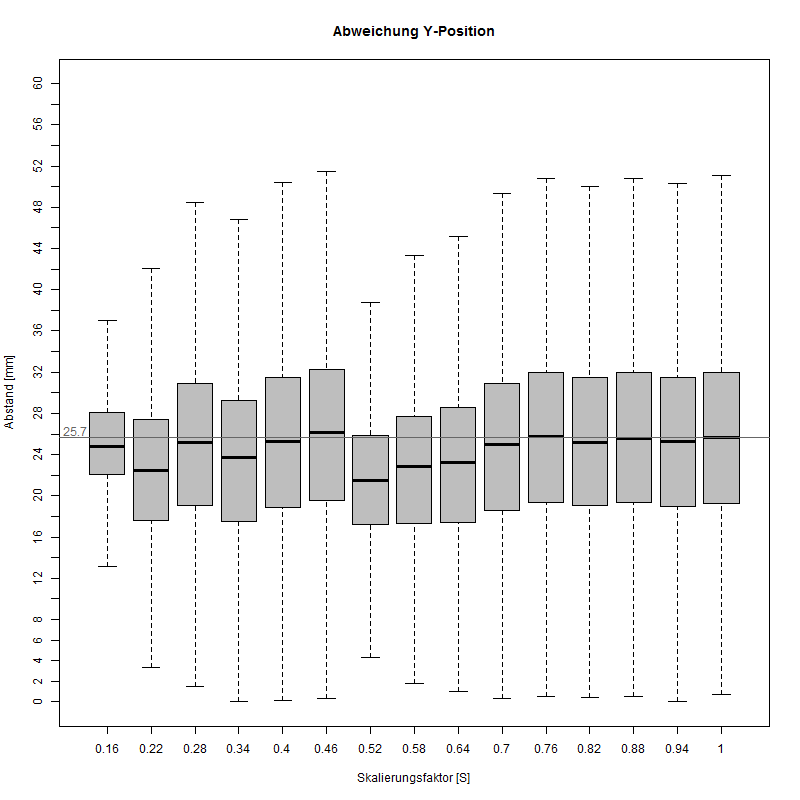
\includegraphics[width=0.245\linewidth]{img_Skalierung/NN_Ty}
	\caption{Zusammenhang zwischen der Skalierung und der Abweichung in Y-Richtung in Millimeter.\\
		Von rechts nach links: Bicubic, Lanczos, Linear, Nearest-Neighbor}
	\label{img_Y_Pos_Skal}
\end{figure}
\begin{figure}
	\centering
	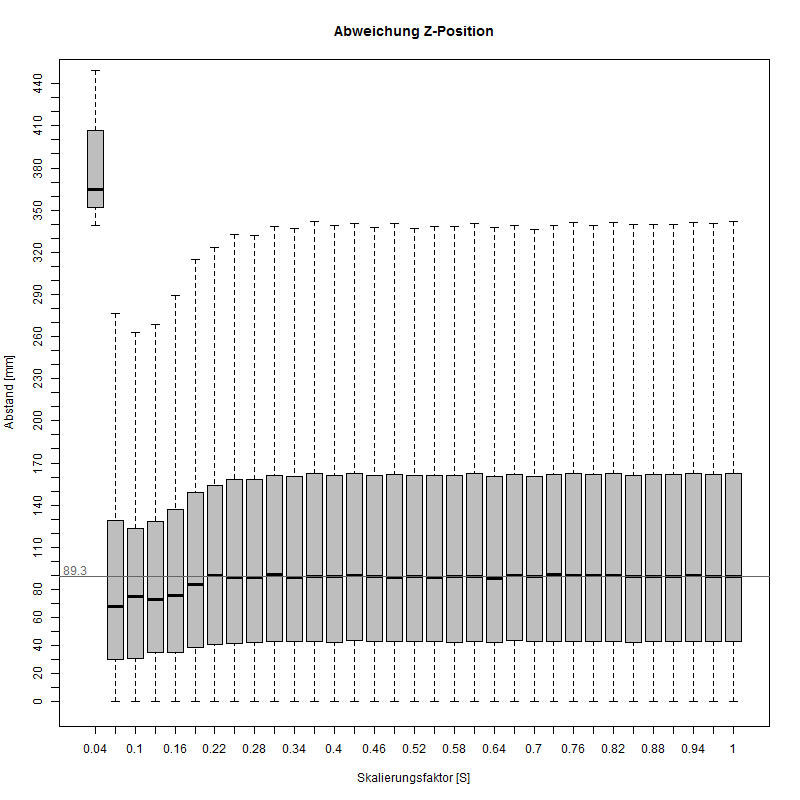
\includegraphics[width=0.245\linewidth]{img_Skalierung/CU_Tz}
	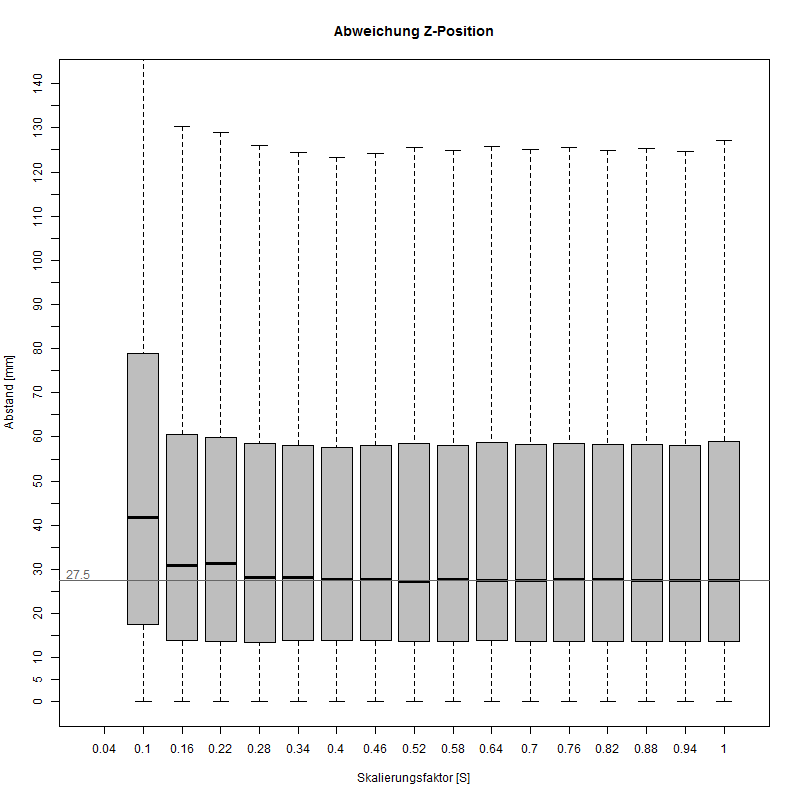
\includegraphics[width=0.245\linewidth]{img_Skalierung/LA_Tz}
	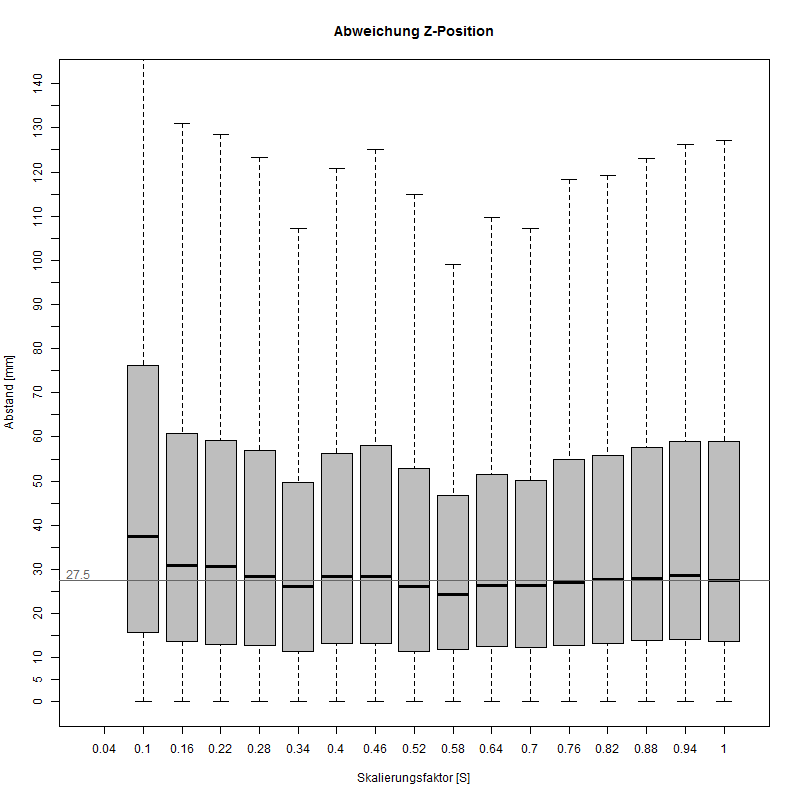
\includegraphics[width=0.245\linewidth]{img_Skalierung/LI_Tz}
	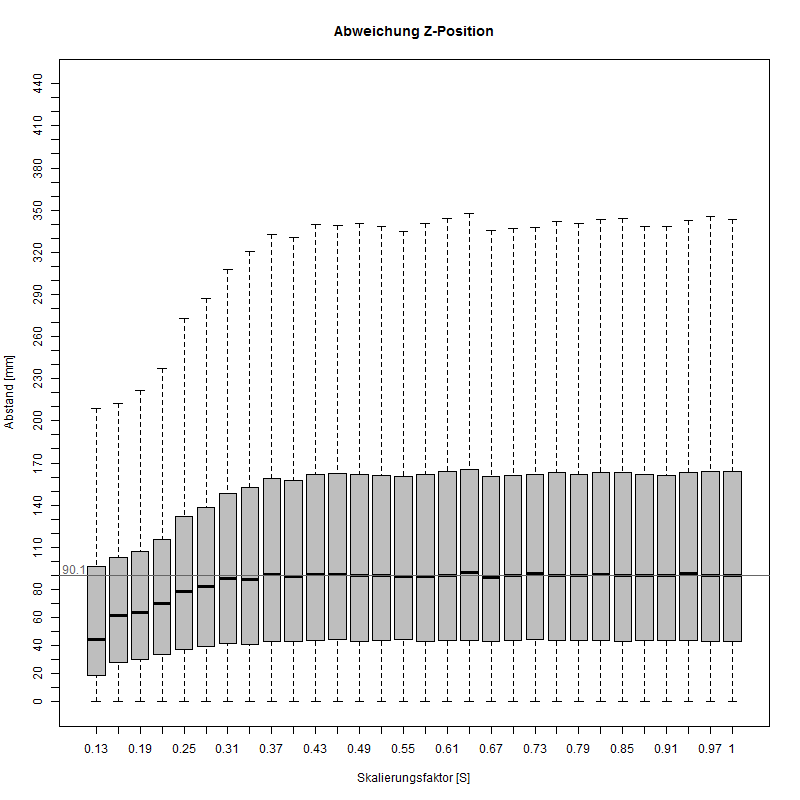
\includegraphics[width=0.245\linewidth]{img_Skalierung/NN_Tz}
	\caption{Zusammenhang zwischen der Skalierung und der Abweichung in Z-Richtung in Millimeter.\\
		Von rechts nach links: Bicubic, Lanczos, Linear, Nearest-Neighbor}
	\label{img_Z_Pos_Skal}
\end{figure}
%-----------------------------------------------------
\begin{figure}
	\centering
	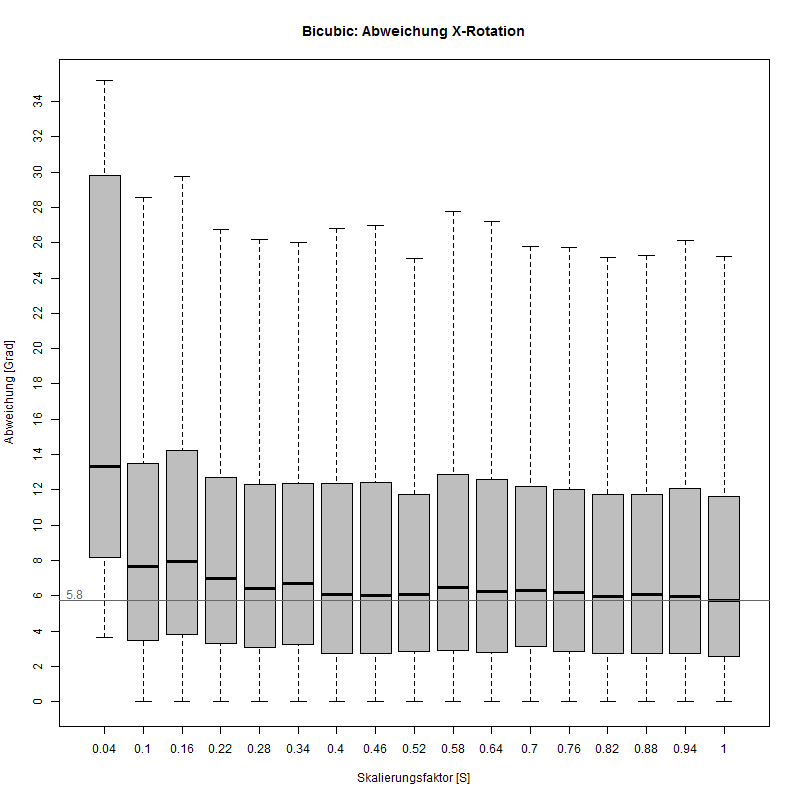
\includegraphics[width=0.245\linewidth]{img_Skalierung/CU_Rx}
	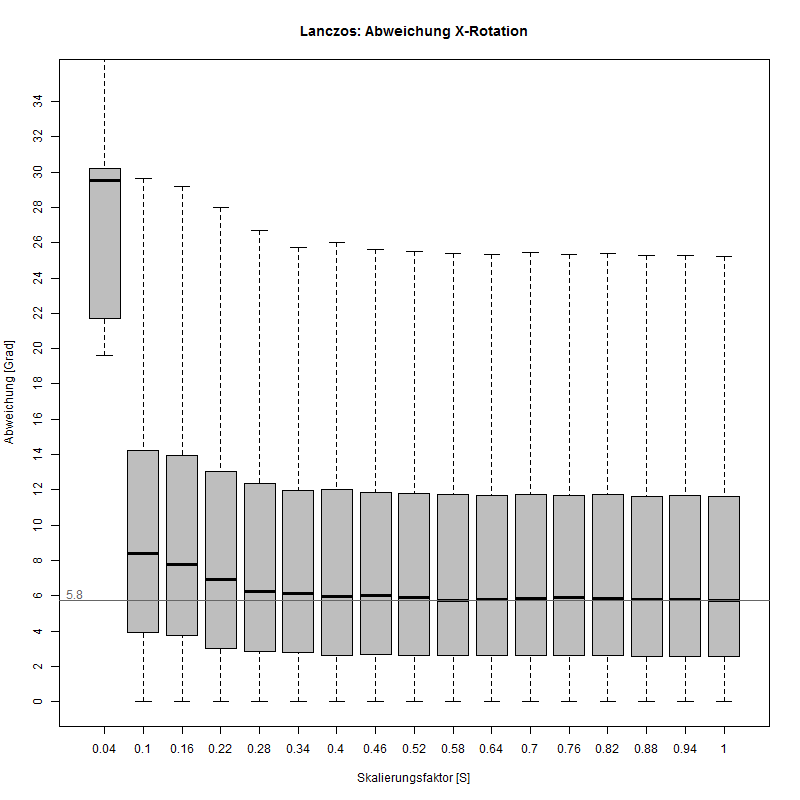
\includegraphics[width=0.245\linewidth]{img_Skalierung/LA_Rx}
	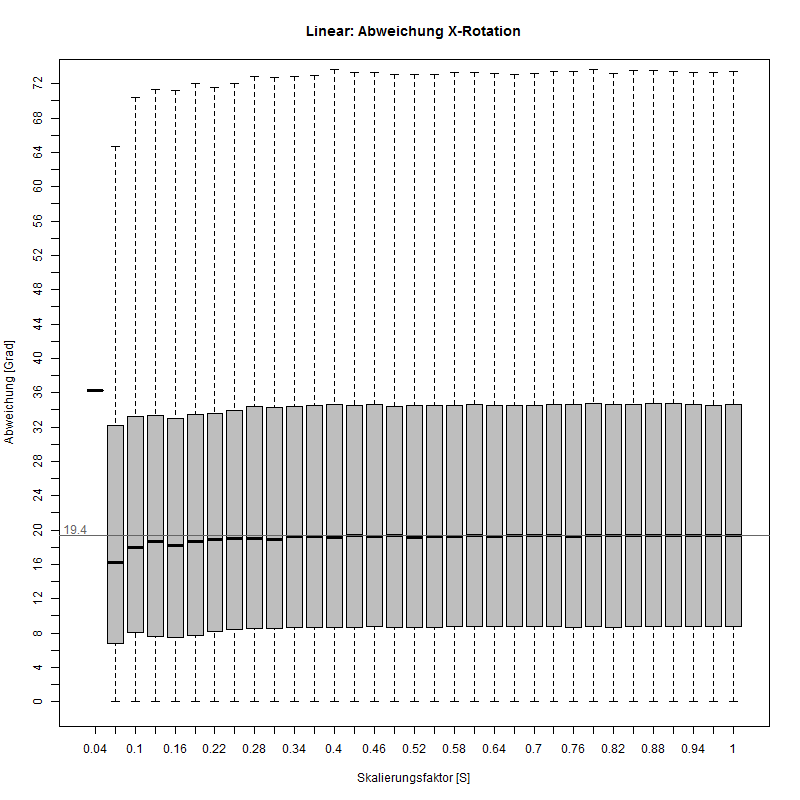
\includegraphics[width=0.245\linewidth]{img_Skalierung/LI_Rx}
	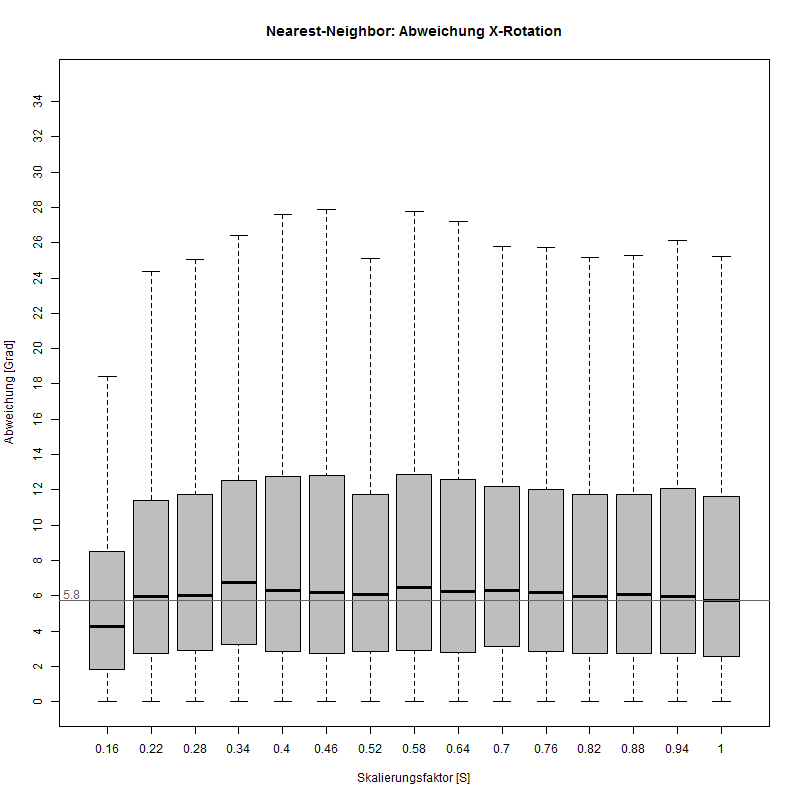
\includegraphics[width=0.245\linewidth]{img_Skalierung/NN_Rx}
	\caption{Zusammenhang zwischen der Skalierung und der Abweichung des Winkels in X-Richtung, Angabe in Bogenmaß.\\
		Von rechts nach links: Bicubic, Lanczos, Linear, Nearest-Neighbor}
	\label{img_X_Rot_Skal}
\end{figure}
\begin{figure}
	\centering
	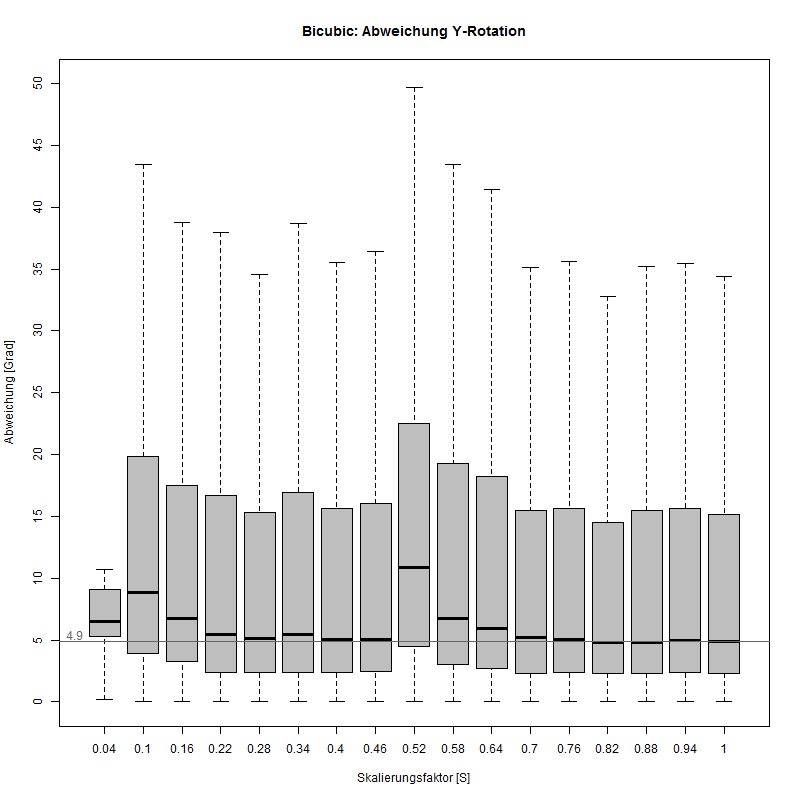
\includegraphics[width=0.245\linewidth]{img_Skalierung/CU_Ry}
	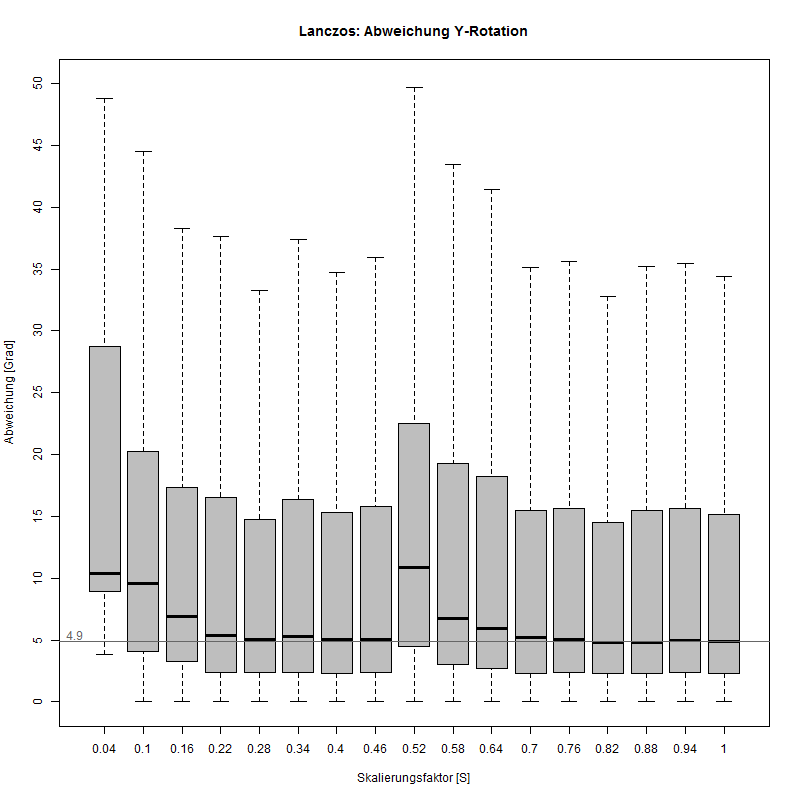
\includegraphics[width=0.245\linewidth]{img_Skalierung/LA_Ry}
	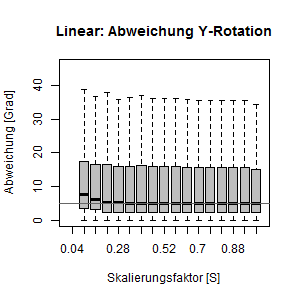
\includegraphics[width=0.245\linewidth]{img_Skalierung/LI_Ry}
	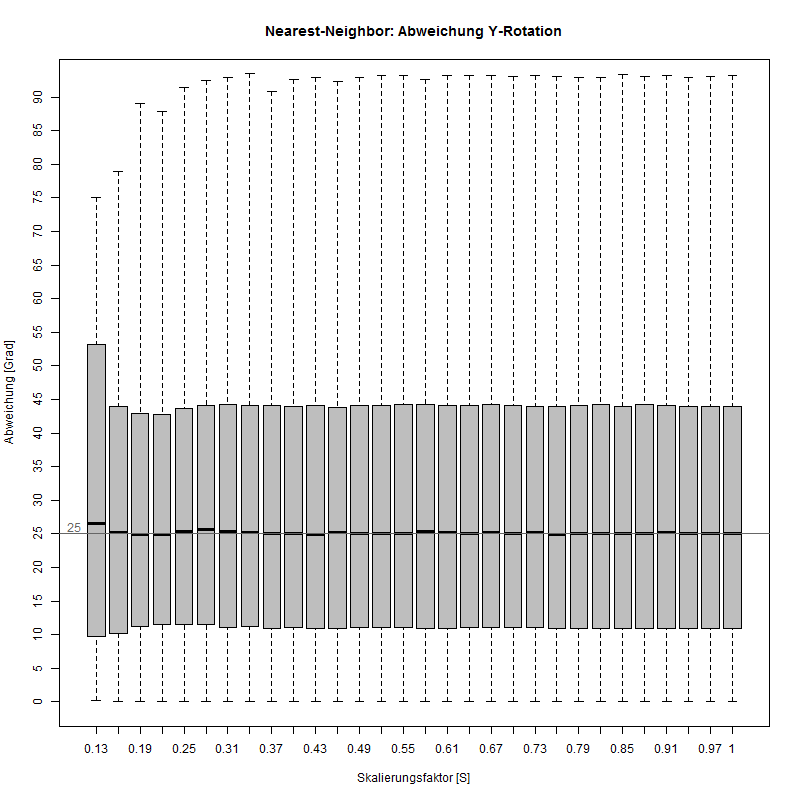
\includegraphics[width=0.245\linewidth]{img_Skalierung/NN_Ry}
	\caption{Zusammenhang zwischen der Skalierung (X-Achse) und der Abweichung des Winkels in X-Richtung, Angabe in Bogenmaß.\\
		Von rechts nach links: Bicubic, Lanczos, Linear, Nearest-Neighbor}
	\label{img_Y_Rot_Skal}
\end{figure}
\begin{figure}
	\centering
	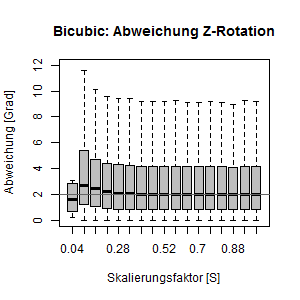
\includegraphics[width=0.245\linewidth]{img_Skalierung/CU_Rz}
	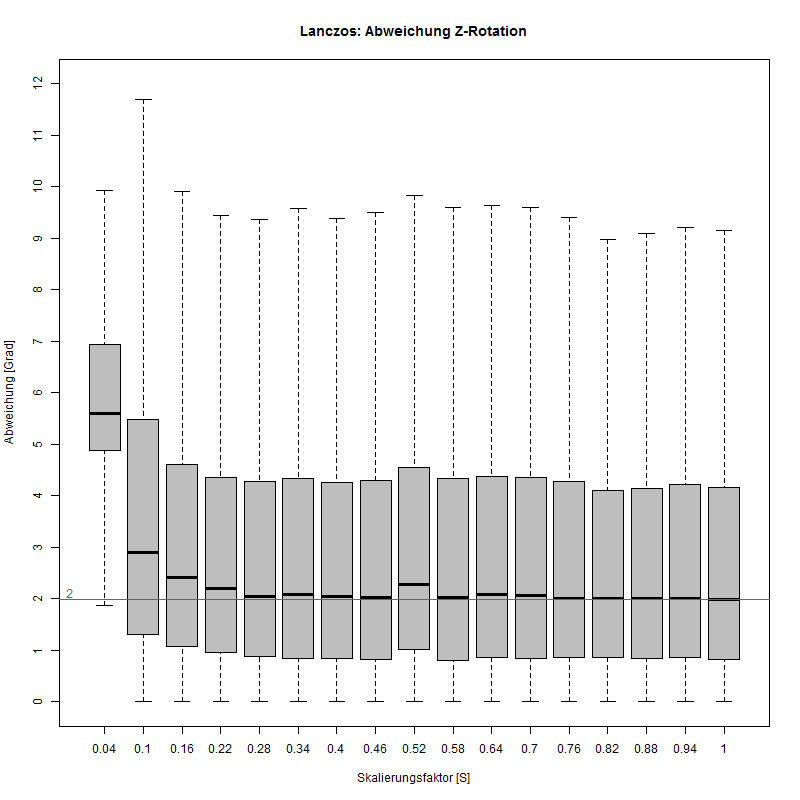
\includegraphics[width=0.245\linewidth]{img_Skalierung/LA_Rz}
	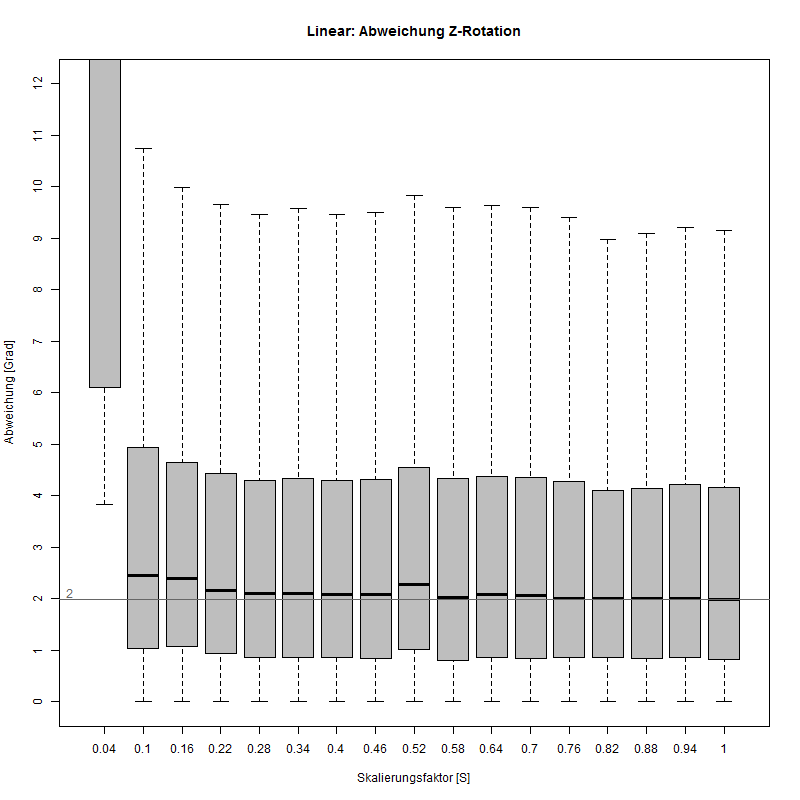
\includegraphics[width=0.245\linewidth]{img_Skalierung/LI_Rz}
	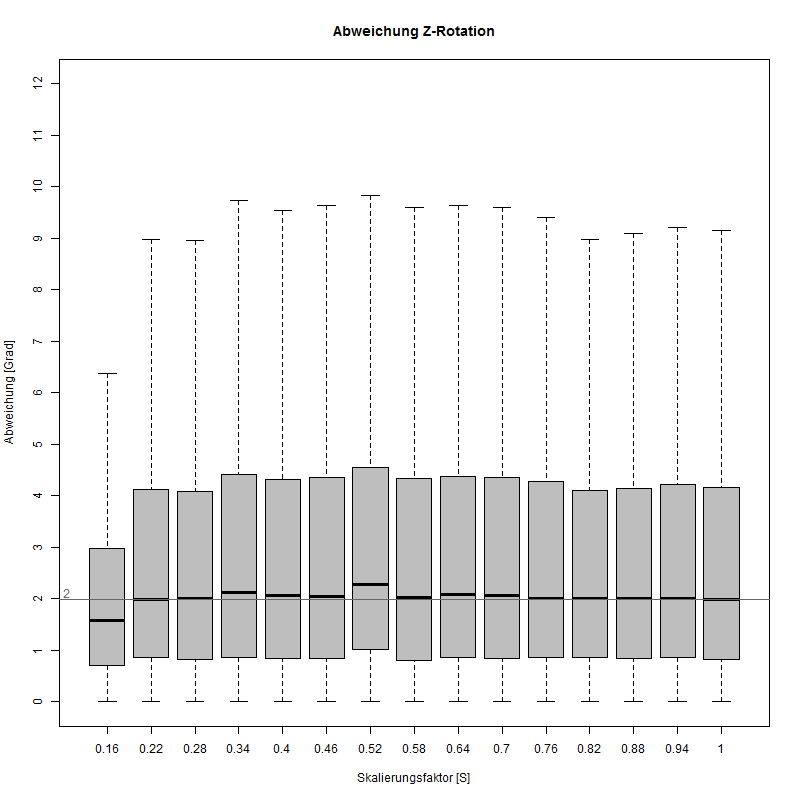
\includegraphics[width=0.245\linewidth]{img_Skalierung/NN_Rz}
	\caption{Zusammenhang zwischen der Skalierung (X-Achse) und der Abweichung des Winkels in Y-Richtung, Angabe in Bogenmaß.\\
		Von rechts nach links: Bicubic, Lanczos, Linear, Nearest-Neighbor}
	\label{img_Z_Rot_Skal}
\end{figure}
\begin{figure}
	\centering
	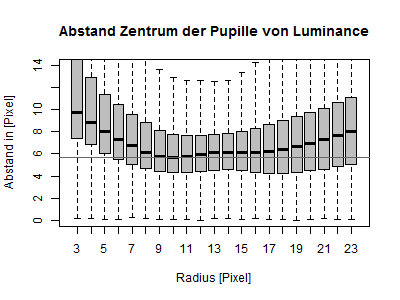
\includegraphics[width=0.32\linewidth]{Eye_Img_Box/Norm_Radius_A}
	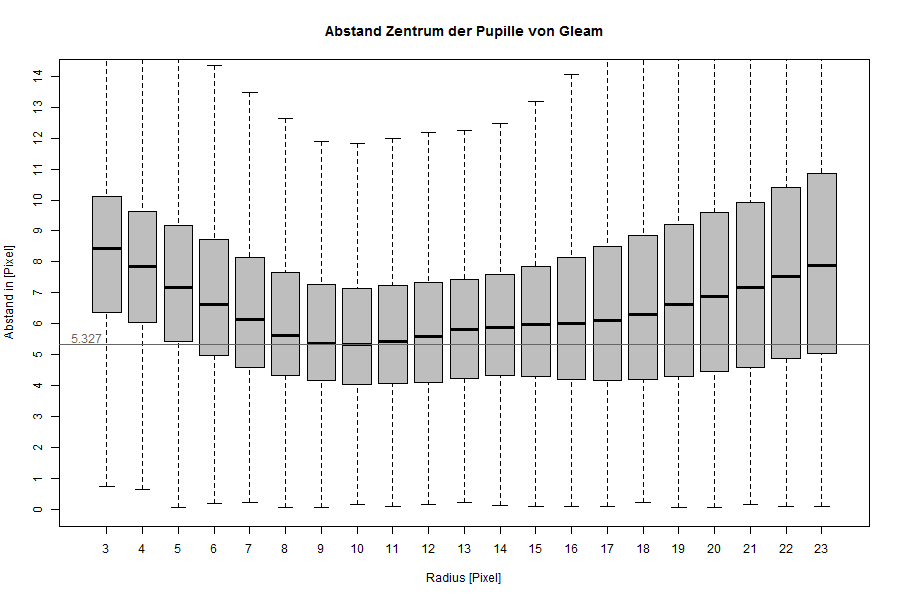
\includegraphics[width=0.32\linewidth]{Eye_Img_Box/Gleam_Radius_A}
	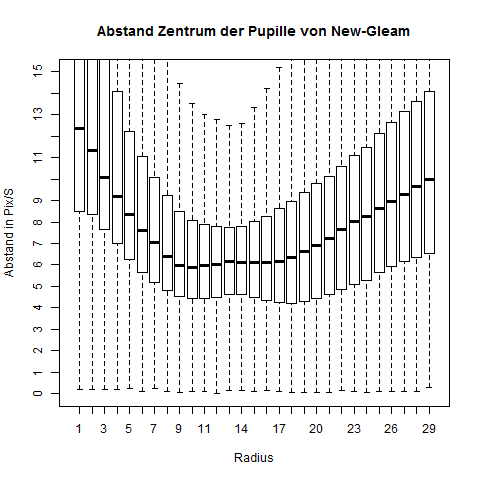
\includegraphics[width=0.32\linewidth]{Eye_Img_Box/New_Radius_A}\\
	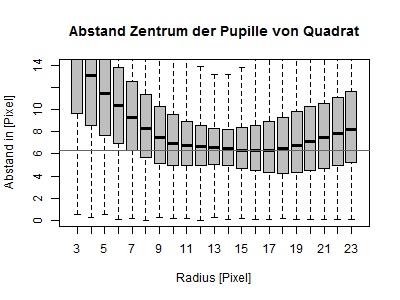
\includegraphics[width=0.32\linewidth]{Eye_Img_Box/Qua_Radius_A}
	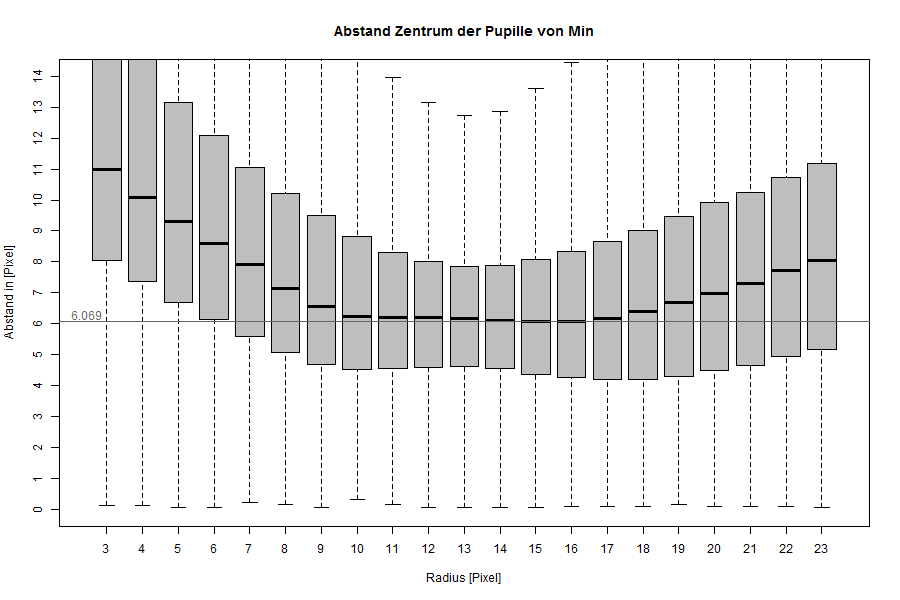
\includegraphics[width=0.32\linewidth]{Eye_Img_Box/Min_Radius_A}
	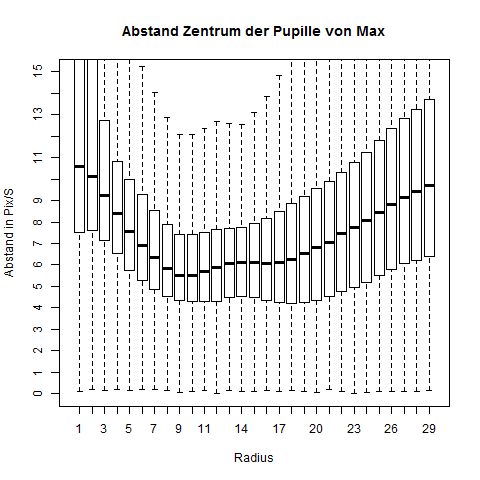
\includegraphics[width=0.32\linewidth]{Eye_Img_Box/Max_Radius_A}
	%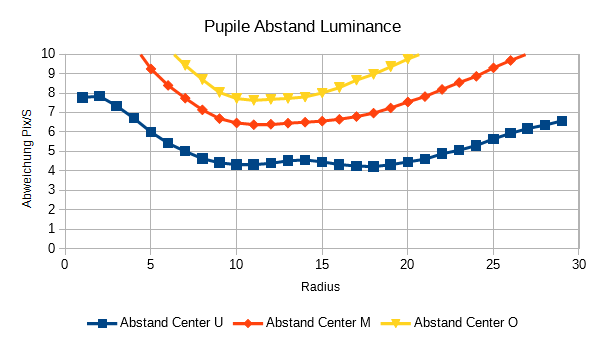
\includegraphics[width=0.49\linewidth]{Eye_Img/Normal_Abstand_P}
	%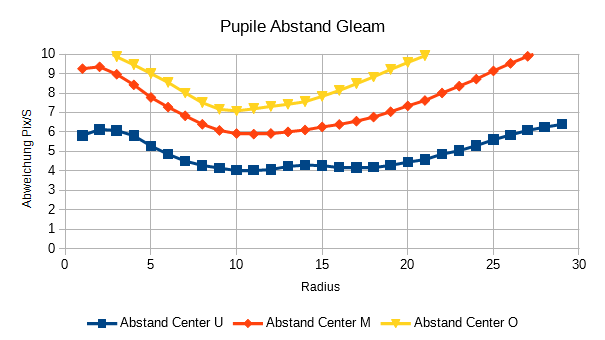
\includegraphics[width=0.49\linewidth]{Eye_Img/Gleam_Abstand_P}
	%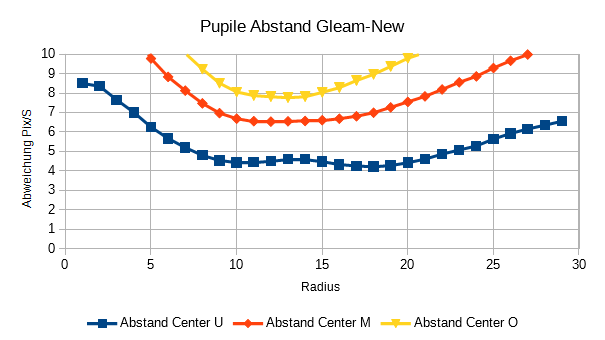
\includegraphics[width=0.49\linewidth]{Eye_Img/New_Abstand_P}
	%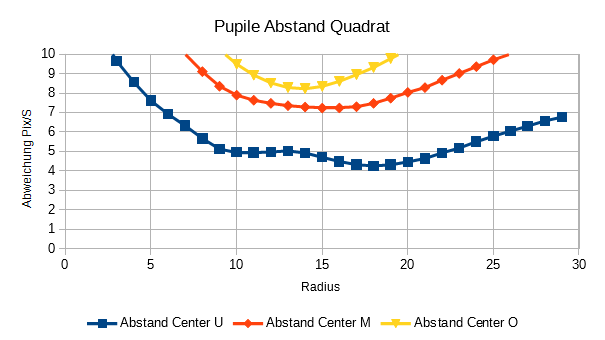
\includegraphics[width=0.49\linewidth]{Eye_Img/Quadrat_Abstand_P}
	%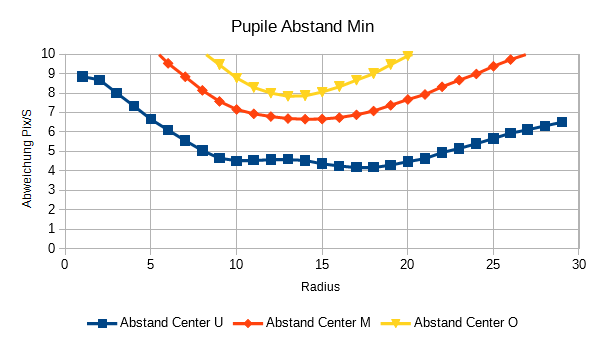
\includegraphics[width=0.49\linewidth]{Eye_Img/Min_Abstand_P}
	%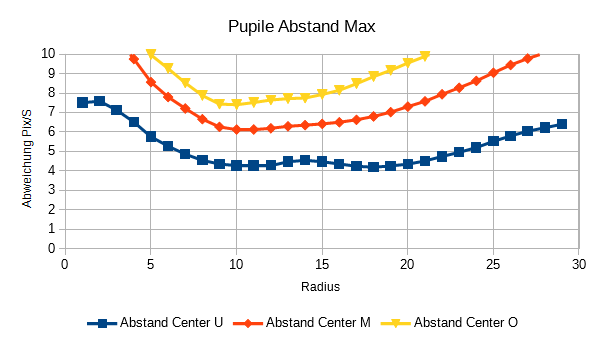
\includegraphics[width=0.49\linewidth]{Eye_Img/Max_Abstand_P}
	\caption{Abstand des Zentrums der Landmark-Pupille und der berechneten Ellipse in [Pixel] gegen den Radius-Größe des Filters.\\
		Oben-Links: Luminance, Oben-Mitte: Gleam, Oben-Rechts: Gleam New,\\ Unten-Links: Quadrat, Unten-Mitte: Min-Wert, Unten-Rechts: Max-Wert}
	\label{ElSe_Gray_Zentrum}
\end{figure}
\begin{figure}
	\centering
	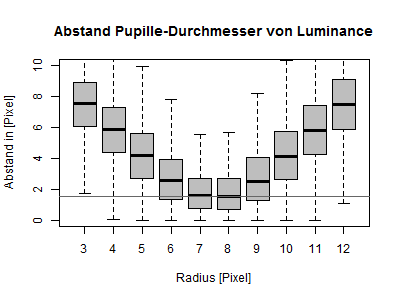
\includegraphics[width=0.32\linewidth]{Eye_Img_Box/Norm_Radius_P}
	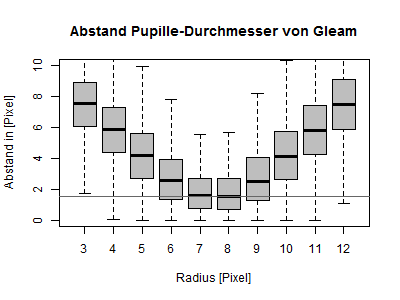
\includegraphics[width=0.32\linewidth]{Eye_Img_Box/Gleam_Radius_P}
	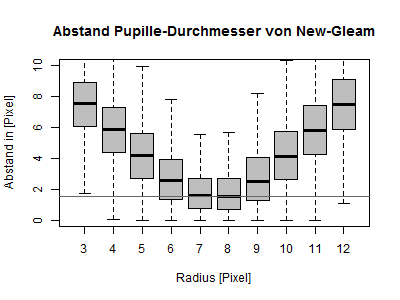
\includegraphics[width=0.32\linewidth]{Eye_Img_Box/New_Radius_P}\\
	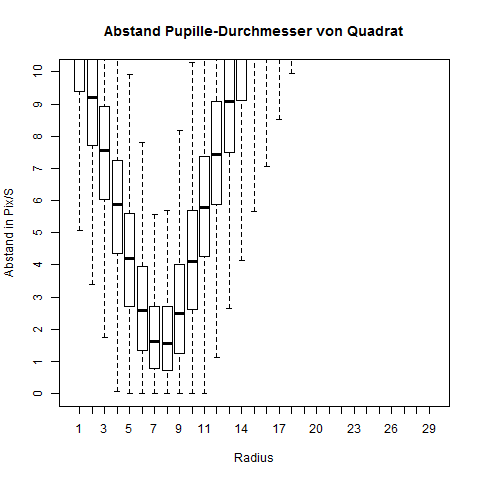
\includegraphics[width=0.32\linewidth]{Eye_Img_Box/Qua_Radius_P}
	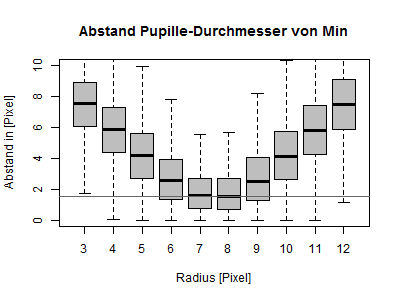
\includegraphics[width=0.32\linewidth]{Eye_Img_Box/Min_Radius_P}
	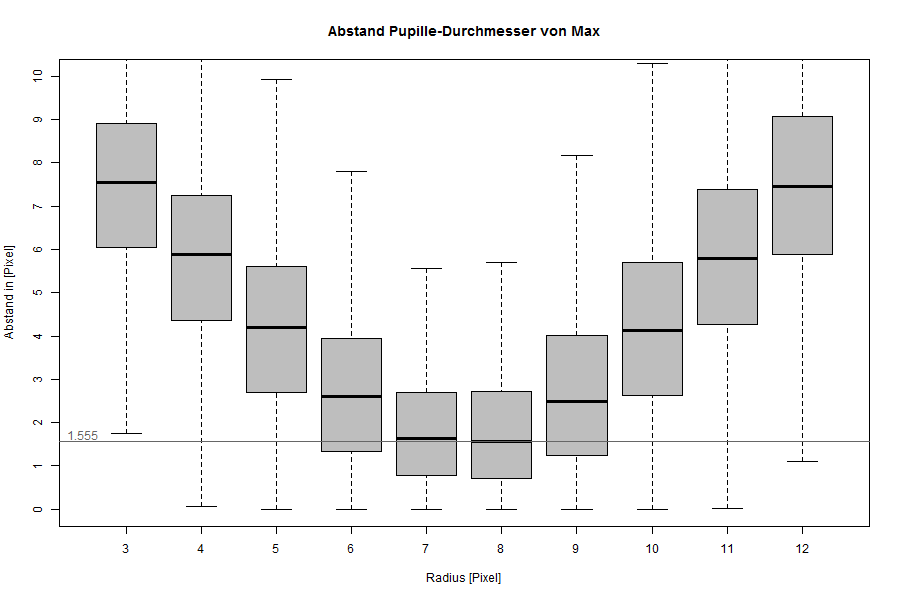
\includegraphics[width=0.32\linewidth]{Eye_Img_Box/Max_Radius_P}
	%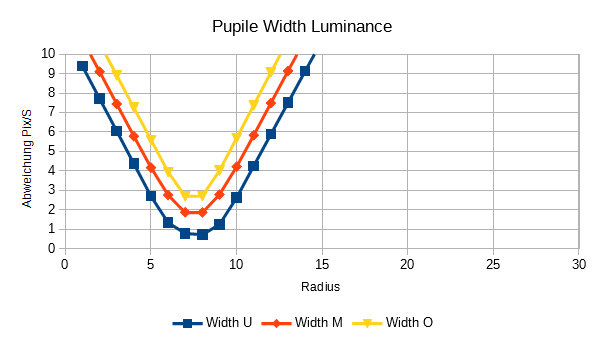
\includegraphics[width=0.49\linewidth]{Eye_Img/Normal_Width_P}
	%\includegraphics[width=0.49\linewidth]{Eye_Img/Gleam_Width_P}
	%\includegraphics[width=0.49\linewidth]{Eye_Img/New_Width_P}
	%\includegraphics[width=0.49\linewidth]{Eye_Img/Quadrat_Width_P}
	%\includegraphics[width=0.49\linewidth]{Eye_Img/Min_Width_P}
	%\includegraphics[width=0.49\linewidth]{Eye_Img/Max_Width_P}
	\caption{Unterschied Zwischen den Radien der Landmark-Pupille und der Berechneten Ellipse in [Pixel] gegen den Radius-Größe des Filters\\
		Oben-Links: Luminance, Oben-Mitte: Gleam, Oben-Rechts: Gleam New,\\ Unten-Links: Quadrat, Unten-Mitte: Min-Wert, Unten-Rechts: Max-Wert}
	\label{ElSe_Gray_Pupille}
\end{figure}
\begin{figure}
	\centering
	\includegraphics[width=0.32\linewidth]{Eye_Img_Box/Norm_Radius_I}
	\includegraphics[width=0.32\linewidth]{Eye_Img_Box/Gleam_Radius_I}
	\includegraphics[width=0.32\linewidth]{Eye_Img_Box/New_Radius_I}\\
	\includegraphics[width=0.32\linewidth]{Eye_Img_Box/Qua_Radius_I}
	\includegraphics[width=0.32\linewidth]{Eye_Img_Box/Min_Radius_I}
	\includegraphics[width=0.32\linewidth]{Eye_Img_Box/Max_Radius_I}
	%\includegraphics[width=0.49\linewidth]{Eye_Img/Normal_Width_I}
	%\includegraphics[width=0.49\linewidth]{Eye_Img/Gleam_Width_I}
	%\includegraphics[width=0.49\linewidth]{Eye_Img/New_Width_I}
	%\includegraphics[width=0.49\linewidth]{Eye_Img/Quadrat_Width_I}
	%\includegraphics[width=0.49\linewidth]{Eye_Img/Min_Width_I}
	%\includegraphics[width=0.49\linewidth]{Eye_Img/Max_Width_I}
	\caption{Unterschied Zwischen den Radien der Landmark-Iris und der Berechneten Ellipse in [Pixel] gegen den Radius-Größe des Filters.\\
		Oben-Links: Luminance, Oben-Mitte: Gleam, Oben-Rechts: Gleam New,\\ Unten-Links: Quadrat, Unten-Mitte: Min-Wert, Unten-Rechts: Max-Wert}
	\label{ElSe_Gray_Iris}
\end{figure}
\begin{figure}
	\centering
	\includegraphics[width=0.32\linewidth]{Eye_Img_Box/Gleam_Radius_P_8}
	\includegraphics[width=0.32\linewidth]{Eye_Img_Box/Norm_Radius_P_8}
	\includegraphics[width=0.32\linewidth]{Eye_Img_Box/Qua_Radius_P_8}\\
	\includegraphics[width=0.32\linewidth]{Eye_Img_Box/Gleam_Radius_A_10}
	\includegraphics[width=0.32\linewidth]{Eye_Img_Box/Norm_Radius_A_10}
	\includegraphics[width=0.32\linewidth]{Eye_Img_Box/Qua_Radius_A_16}\\
	\includegraphics[width=0.32\linewidth]{Eye_Img_Box/Gleam_Radius_I_18}
	\includegraphics[width=0.32\linewidth]{Eye_Img_Box/Norm_Radius_I_18}
	\includegraphics[width=0.32\linewidth]{Eye_Img_Box/Qua_Radius_I_18}
	\caption{Auswirkung von der Bildgröße auf die Qualität der Berechnung. Aufgetragen ist die Abweichung [Pixel/Skalierung] gegen den Skalierungsfaktor. Oben: Pupille-Durchmesser, Mitte Abweichung Zentrum, Iris-Durchmesser\\
		Links: Gleam, Mitte: Luminance, Rechts Quadrat}
	\label{ElSe_scall}
\end{figure}
\end{landscape}
\begin{figure}
	\centering
	\includegraphics[width=0.49\linewidth]{Eye_Img_Box/Openface_BoxX}
	\includegraphics[width=0.49\linewidth]{Eye_Img_Box/Openface_BoxY}\\
	\includegraphics[width=0.49\linewidth]{Eye_Img_Box/Openface_BoxW}
	\includegraphics[width=0.49\linewidth]{Eye_Img_Box/Openface_BoxH}
	%\includegraphics[width=0.245\linewidth]{Eye_Img/Box_X}
	%\includegraphics[width=0.245\linewidth]{Eye_Img/Box_Y}
	%\includegraphics[width=0.245\linewidth]{Eye_Img/Box_W}
	%\includegraphics[width=0.245\linewidth]{Eye_Img/Box_H}
	\caption{Bestimmung der Box ums Auge abhängig von der Bildgröße. Aufgetragen ist die Abweichung [Pixel/Skalierung] gegen den Skalierungsfaktor.\\
		Dargestellt sind Koordinaten, X- und Y-Position in Pixel sowie die Ausdehnung der Box (Width und Hight) ebenfalls in Pixel relativ zur umschließenden Box der Landmarks.}
	\label{OpenFace_Eye_Box}
\end{figure}
\begin{landscape}
	\begin{figure}
		\centering
		\includegraphics[width=0.192\linewidth]{OpenFace_Img/Head_x_Err_S1}
		\includegraphics[width=0.192\linewidth]{OpenFace_Img/Head_x_Err_S05}
		\includegraphics[width=0.192\linewidth]{OpenFace_Img/Head_x_Err_S025}
		\includegraphics[width=0.192\linewidth]{OpenFace_Img/Head_x_Err_S01}
		\includegraphics[width=0.192\linewidth]{OpenFace_Img/Head_x_Err_S005}\\	
		\includegraphics[width=0.192\linewidth]{OpenFace_Img/Head_y_Err_S1}
		\includegraphics[width=0.192\linewidth]{OpenFace_Img/Head_y_Err_S05}
		\includegraphics[width=0.192\linewidth]{OpenFace_Img/Head_y_Err_S025}
		\includegraphics[width=0.192\linewidth]{OpenFace_Img/Head_y_Err_S01}
		\includegraphics[width=0.192\linewidth]{OpenFace_Img/Head_y_Err_S005}\\	
		\includegraphics[width=0.192\linewidth]{OpenFace_Img/EyeAVG_x_Err_S1}	
		\includegraphics[width=0.192\linewidth]{OpenFace_Img/EyeAVG_x_Err_S05}
		\includegraphics[width=0.192\linewidth]{OpenFace_Img/EyeAVG_x_Err_S025}
		\includegraphics[width=0.192\linewidth]{OpenFace_Img/EyeAVG_x_Err_S01}
		\includegraphics[width=0.192\linewidth]{OpenFace_Img/EyeAVG_x_Err_S005}
		\caption{Abweichung der Videoaufnahme von der Kopfausrichtung Horizontal (Oben), Kopforientierung Vertikal (Mitte) und die X-Ausrichtung der Augen (Unten)\\Skalierungsfaktor von links nach rechts (1/0.5/0.25/0.1/0.05), Y-Achse: $[0-35]^\circ$}
		\label{graph_VideoSkalierung_Err}
	\end{figure}
\end{landscape}
\begin{figure}
	\centering
		\begin{tabular}{|c|c|c|c|c|c|c|c|}
	\hline
	$+11m$ & & & &
	\includegraphics[width=1cm]{img_Bereich/V1_img_res_Winkel_X_0_11000.png}& & &\\ 
	\hline 
	$+10m$ &
	\includegraphics[width=1cm]{img_Bereich/V1_img_res_Winkel_X_-3000_10000.png} &
	\includegraphics[width=1cm]{img_Bereich/V1_img_res_Winkel_X_-2000_10000.png}&
	\includegraphics[width=1cm]{img_Bereich/V1_img_res_Winkel_X_-1000_10000.png}&
	\includegraphics[width=1cm]{img_Bereich/V1_img_res_Winkel_X_0_10000.png}&
	\includegraphics[width=1cm]{img_Bereich/V1_img_res_Winkel_X_1000_10000.png}&
	\includegraphics[width=1cm]{img_Bereich/V1_img_res_Winkel_X_2000_10000.png}&
	\includegraphics[width=1cm]{img_Bereich/V1_img_res_Winkel_X_3000_10000.png}\\ 
	\hline 
	$+9m$ &
	\includegraphics[width=1cm]{img_Bereich/V1_img_res_Winkel_X_-3000_9000.png} &
	\includegraphics[width=1cm]{img_Bereich/V1_img_res_Winkel_X_-2000_9000.png}&
	\includegraphics[width=1cm]{img_Bereich/V1_img_res_Winkel_X_-1000_9000.png}&
	\includegraphics[width=1cm]{img_Bereich/V1_img_res_Winkel_X_0_9000.png}&
	\includegraphics[width=1cm]{img_Bereich/V1_img_res_Winkel_X_1000_9000.png}&
	\includegraphics[width=1cm]{img_Bereich/V1_img_res_Winkel_X_2000_9000.png}&
	\includegraphics[width=1cm]{img_Bereich/V1_img_res_Winkel_X_3000_9000.png}\\ 
	\hline 
	$+8m$ &
	\includegraphics[width=1cm]{img_Bereich/V1_img_res_Winkel_X_-3000_8000.png} &
	\includegraphics[width=1cm]{img_Bereich/V1_img_res_Winkel_X_-2000_8000.png}&
	\includegraphics[width=1cm]{img_Bereich/V1_img_res_Winkel_X_-1000_8000.png}&
	\includegraphics[width=1cm]{img_Bereich/V1_img_res_Winkel_X_0_8000.png}&
	\includegraphics[width=1cm]{img_Bereich/V1_img_res_Winkel_X_1000_8000.png}&
	\includegraphics[width=1cm]{img_Bereich/V1_img_res_Winkel_X_2000_8000.png}&
	\includegraphics[width=1cm]{img_Bereich/V1_img_res_Winkel_X_3000_8000.png}\\ 
	\hline 
	$+7m$ &
	\includegraphics[width=1cm]{img_Bereich/V1_img_res_Winkel_X_-3000_7000.png} &
	\includegraphics[width=1cm]{img_Bereich/V1_img_res_Winkel_X_-2000_7000.png}&
	\includegraphics[width=1cm]{img_Bereich/V1_img_res_Winkel_X_-1000_7000.png}&
	\includegraphics[width=1cm]{img_Bereich/V1_img_res_Winkel_X_0_7000.png}&
	\includegraphics[width=1cm]{img_Bereich/V1_img_res_Winkel_X_1000_7000.png}&
	\includegraphics[width=1cm]{img_Bereich/V1_img_res_Winkel_X_2000_7000.png}&
	\includegraphics[width=1cm]{img_Bereich/V1_img_res_Winkel_X_3000_7000.png}\\ 
	\hline 
	$+6m$ &
	\includegraphics[width=1cm]{img_Bereich/V1_img_res_Winkel_X_-3000_6000.png} &
	\includegraphics[width=1cm]{img_Bereich/V1_img_res_Winkel_X_-2000_6000.png}&
	\includegraphics[width=1cm]{img_Bereich/V1_img_res_Winkel_X_-1000_6000.png}&
	\includegraphics[width=1cm]{img_Bereich/V1_img_res_Winkel_X_0_6000.png}&
	\includegraphics[width=1cm]{img_Bereich/V1_img_res_Winkel_X_1000_6000.png}&
	\includegraphics[width=1cm]{img_Bereich/V1_img_res_Winkel_X_2000_6000.png}&
	\includegraphics[width=1cm]{img_Bereich/V1_img_res_Winkel_X_3000_6000.png}\\ 
	\hline 
	$+5m$ &
	\includegraphics[width=1cm]{img_Bereich/V1_img_res_Winkel_X_-3000_5000.png}&
	\includegraphics[width=1cm]{img_Bereich/V1_img_res_Winkel_X_-2000_5000.png}&
	\includegraphics[width=1cm]{img_Bereich/V1_img_res_Winkel_X_-1000_5000.png}&
	\includegraphics[width=1cm]{img_Bereich/V1_img_res_Winkel_X_0_5000.png}&
	\includegraphics[width=1cm]{img_Bereich/V1_img_res_Winkel_X_1000_5000.png}&
	\includegraphics[width=1cm]{img_Bereich/V1_img_res_Winkel_X_2000_5000.png}&
	\includegraphics[width=1cm]{img_Bereich/V1_img_res_Winkel_X_3000_5000.png}\\ 
	\hline 
	$+4m$ &
	\includegraphics[width=1cm]{img_Bereich/V1_img_res_Winkel_X_-3000_4000.png}&
	\includegraphics[width=1cm]{img_Bereich/V1_img_res_Winkel_X_-2000_4000.png} &
	\includegraphics[width=1cm]{img_Bereich/V1_img_res_Winkel_X_-1000_4000.png}&
	\includegraphics[width=1cm]{img_Bereich/V1_img_res_Winkel_X_0_4000.png}&
	\includegraphics[width=1cm]{img_Bereich/V1_img_res_Winkel_X_1000_4000.png}&
	\includegraphics[width=1cm]{img_Bereich/V1_img_res_Winkel_X_2000_4000.png}&\\ 
	\hline 
	$+3m$ & &
	\includegraphics[width=1cm]{img_Bereich/V1_img_res_Winkel_X_-2000_3000.png} &
	\includegraphics[width=1cm]{img_Bereich/V1_img_res_Winkel_X_-1000_3000.png}&
	\includegraphics[width=1cm]{img_Bereich/V1_img_res_Winkel_X_0_3000.png}&
	\includegraphics[width=1cm]{img_Bereich/V1_img_res_Winkel_X_1000_3000.png}&
	\includegraphics[width=1cm]{img_Bereich/V1_img_res_Winkel_X_2000_3000.png}& \\ 
	\hline 
	$+2m$ & & &
	\includegraphics[width=1cm]{img_Bereich/V1_img_res_Winkel_X_-1000_2000.png}&
	\includegraphics[width=1cm]{img_Bereich/V1_img_res_Winkel_X_0_2000.png}&
	\includegraphics[width=1cm]{img_Bereich/V1_img_res_Winkel_X_1000_2000.png}& &\\ 
	\hline 
	$+1m$ & & &
	\includegraphics[width=1cm]{img_Bereich/V1_img_res_Winkel_X_-1000_1000.png}&
	\includegraphics[width=1cm]{img_Bereich/V1_img_res_Winkel_X_0_1000.png}&
	\includegraphics[width=1cm]{img_Bereich/V1_img_res_Winkel_X_1000_1000.png}& &\\ 
	\hline 
	& $-3m$ & $-2m$ & $-1m$ &Kamera& $+1m$ & $+2m$ & $+3m$ \\ 
	\hline 
\end{tabular}
		\begin{tabular}{|c|c|c|c|c|c|c|c|}
	\hline
	$+11m$ & & & &
	\includegraphics[width=1cm]{img_Bereich/V1_vid_res_Winkel_X_0_11000.png}& & &\\ 
	\hline 
	$+10m$ & & &
	\includegraphics[width=1cm]{img_Bereich/V1_vid_res_Winkel_X_-1000_10000.png}&
	\includegraphics[width=1cm]{img_Bereich/V1_vid_res_Winkel_X_0_10000.png}&
	\includegraphics[width=1cm]{img_Bereich/V1_vid_res_Winkel_X_1000_10000.png}&
	\includegraphics[width=1cm]{img_Bereich/V1_vid_res_Winkel_X_2000_10000.png}&\\ 
	\hline 
	$+9m$ & & &
	\includegraphics[width=1cm]{img_Bereich/V1_vid_res_Winkel_X_-1000_9000.png}&
	\includegraphics[width=1cm]{img_Bereich/V1_vid_res_Winkel_X_0_9000.png}&
	\includegraphics[width=1cm]{img_Bereich/V1_vid_res_Winkel_X_1000_9000.png}&
	\includegraphics[width=1cm]{img_Bereich/V1_vid_res_Winkel_X_2000_9000.png}&\\ 
	\hline 
	$+8m$ & & &
	\includegraphics[width=1cm]{img_Bereich/V1_vid_res_Winkel_X_-1000_8000.png}&
	\includegraphics[width=1cm]{img_Bereich/V1_vid_res_Winkel_X_0_8000.png}&
	\includegraphics[width=1cm]{img_Bereich/V1_vid_res_Winkel_X_1000_8000.png}& & \\ 
	\hline 
	$+7m$ & & &
	\includegraphics[width=1cm]{img_Bereich/V1_vid_res_Winkel_X_-1000_7000.png}&
	\includegraphics[width=1cm]{img_Bereich/V1_vid_res_Winkel_X_0_7000.png}&
	\includegraphics[width=1cm]{img_Bereich/V1_vid_res_Winkel_X_1000_7000.png}& & \\ 
	\hline 
	$+6m$ & & &
	\includegraphics[width=1cm]{img_Bereich/V1_vid_res_Winkel_X_-1000_6000.png}&
	\includegraphics[width=1cm]{img_Bereich/V1_vid_res_Winkel_X_0_6000.png}&
	\includegraphics[width=1cm]{img_Bereich/V1_vid_res_Winkel_X_1000_6000.png}&
	\includegraphics[width=1cm]{img_Bereich/V1_vid_res_Winkel_X_2000_6000.png}&
	\includegraphics[width=1cm]{img_Bereich/V1_vid_res_Winkel_X_3000_6000.png}\\ 
	\hline 
	$+5m$ &
	\includegraphics[width=1cm]{img_Bereich/V1_vid_res_Winkel_X_-3000_5000.png}& &
	\includegraphics[width=1cm]{img_Bereich/V1_vid_res_Winkel_X_-1000_5000.png}&
	\includegraphics[width=1cm]{img_Bereich/V1_vid_res_Winkel_X_0_5000.png}&
	\includegraphics[width=1cm]{img_Bereich/V1_vid_res_Winkel_X_1000_5000.png}&
	\includegraphics[width=1cm]{img_Bereich/V1_vid_res_Winkel_X_2000_5000.png}&
	\includegraphics[width=1cm]{img_Bereich/V1_vid_res_Winkel_X_3000_5000.png}\\ 
	\hline 
	$+4m$ &
	\includegraphics[width=1cm]{img_Bereich/V1_vid_res_Winkel_X_-3000_4000.png}& &
	\includegraphics[width=1cm]{img_Bereich/V1_vid_res_Winkel_X_-1000_4000.png}&
	\includegraphics[width=1cm]{img_Bereich/V1_vid_res_Winkel_X_0_4000.png}&
	\includegraphics[width=1cm]{img_Bereich/V1_vid_res_Winkel_X_1000_4000.png}&
	\includegraphics[width=1cm]{img_Bereich/V1_vid_res_Winkel_X_2000_4000.png}&
	\includegraphics[width=1cm]{img_Bereich/V1_vid_res_Winkel_X_3000_4000.png}\\ 
	\hline 
	$+3m$ &
	\includegraphics[width=1cm]{img_Bereich/V1_vid_res_Winkel_X_-3000_3000.png}& &
	\includegraphics[width=1cm]{img_Bereich/V1_vid_res_Winkel_X_-1000_3000.png}&
	\includegraphics[width=1cm]{img_Bereich/V1_vid_res_Winkel_X_0_3000.png}&
	\includegraphics[width=1cm]{img_Bereich/V1_vid_res_Winkel_X_1000_3000.png}&
	\includegraphics[width=1cm]{img_Bereich/V1_vid_res_Winkel_X_2000_3000.png}&
	\includegraphics[width=1cm]{img_Bereich/V1_vid_res_Winkel_X_3000_3000.png}\\ 
	\hline 
	$+2m$ & & &
	\includegraphics[width=1cm]{img_Bereich/V1_vid_res_Winkel_X_-1000_2000.png}&
	\includegraphics[width=1cm]{img_Bereich/V1_vid_res_Winkel_X_0_2000.png}&
	\includegraphics[width=1cm]{img_Bereich/V1_vid_res_Winkel_X_1000_2000.png}&
	\includegraphics[width=1cm]{img_Bereich/V1_vid_res_Winkel_X_2000_2000.png}&\\ 
	\hline 
	$+1m$ & & &
	\includegraphics[width=1cm]{img_Bereich/V1_vid_res_Winkel_X_-1000_1000.png}&
	\includegraphics[width=1cm]{img_Bereich/V1_vid_res_Winkel_X_0_1000.png}&
	\includegraphics[width=1cm]{img_Bereich/V1_vid_res_Winkel_X_1000_1000.png}& &\\ 
	\hline 
	& $-3m$ & $-2m$ & $-1m$ &Kamera& $+1m$ & $+2m$ & $+3m$ \\ 
	\hline 
\end{tabular}
	\caption{Dargestellt ist der horizontale Winkelbereich in denen ein Gesicht mit aufbereitetem Inhalt erkannt wurde.\\
		Links: Einzelbilder, Rechts: Video}
	\label{graph_Test_1_Resize}
\end{figure}
\begin{landscape}
\begin{figure}
	\centering
	\begin{tabular}{|c|c|c|c|c|c|c|c|}
\hline 
$+12m$&&&
\includegraphics[width=0.115\linewidth]{Auge1/A_Img12-3FalkoE.png} &
\includegraphics[width=0.115\linewidth]{Auge1/A_Img12-4FalkoE.png}  &
\includegraphics[width=0.115\linewidth]{Auge1/A_Img12-5FalkoE.png} && \\ 
&&&&
\includegraphics[width=0.115\linewidth]{Auge1/A_Img12-4ThomasE.png}  &
\includegraphics[width=0.115\linewidth]{Auge1/A_Img12-5ThomasE.png} && \\ \hline 
$+11m$&&&
\includegraphics[width=0.115\linewidth]{Auge1/A_Img11-3FalkoE.png} &
\includegraphics[width=0.115\linewidth]{Auge1/A_Img11-4FalkoE.png} &
\tabbild[width=0.115\linewidth]{Auge1/A_Img11-5FalkoE.png} &
&
\\
&&&
\includegraphics[width=0.115\linewidth]{Auge1/A_Img11-3ThomasE.png} &
\includegraphics[width=0.115\linewidth]{Auge1/A_Img11-4ThomasE.png} &
\includegraphics[width=0.115\linewidth]{Auge1/A_Img11-5ThomasE.png} &
&\\\hline 
$+10m$&
\includegraphics[width=0.115\linewidth]{Auge1/A_Img10-1FalkoE.png} &
\includegraphics[width=0.115\linewidth]{Auge1/A_Img10-2FalkoE.png} &
\includegraphics[width=0.115\linewidth]{Auge1/A_Img10-3FalkoE.png} &
\includegraphics[width=0.115\linewidth]{Auge1/A_Img10-4FalkoE.png} &
\tabbild[width=0.115\linewidth]{Auge1/A_Img10-5FalkoE.png} &
\includegraphics[width=0.115\linewidth]{Auge1/A_Img10-6FalkoE.png} &
\includegraphics[width=0.115\linewidth]{Auge1/A_Img10-7FalkoE.png} \\&
\includegraphics[width=0.115\linewidth]{Auge1/A_Img10-1ThomasE.png} &
\includegraphics[width=0.115\linewidth]{Auge1/A_Img10-2ThomasE.png} &
\includegraphics[width=0.115\linewidth]{Auge1/A_Img10-3ThomasE.png} &
\includegraphics[width=0.115\linewidth]{Auge1/A_Img10-4ThomasE.png} &
\includegraphics[width=0.115\linewidth]{Auge1/A_Img10-5ThomasE.png} &
\includegraphics[width=0.115\linewidth]{Auge1/A_Img10-6ThomasE.png} &
\includegraphics[width=0.115\linewidth]{Auge1/A_Img10-7ThomasE.png} \\\hline 
$+9m$&
\includegraphics[width=0.115\linewidth]{Auge1/A_Img9-1FalkoE.png} &
\includegraphics[width=0.115\linewidth]{Auge1/A_Img9-2FalkoE.png} &
\includegraphics[width=0.115\linewidth]{Auge1/A_Img9-3FalkoE.png} &
\includegraphics[width=0.115\linewidth]{Auge1/A_Img9-4FalkoE.png} &
\tabbild[width=0.115\linewidth]{Auge1/A_Img9-5FalkoE.png} &
\includegraphics[width=0.115\linewidth]{Auge1/A_Img9-6FalkoE.png} &
\includegraphics[width=0.115\linewidth]{Auge1/A_Img9-7FalkoE.png} \\&
\includegraphics[width=0.115\linewidth]{Auge1/A_Img9-1ThomasE.png} &
\includegraphics[width=0.115\linewidth]{Auge1/A_Img9-2ThomasE.png} &
\includegraphics[width=0.115\linewidth]{Auge1/A_Img9-3ThomasE.png} &
\includegraphics[width=0.115\linewidth]{Auge1/A_Img9-4ThomasE.png} &
\includegraphics[width=0.115\linewidth]{Auge1/A_Img9-5ThomasE.png} &
\includegraphics[width=0.115\linewidth]{Auge1/A_Img9-6ThomasE.png} &
\includegraphics[width=0.115\linewidth]{Auge1/A_Img9-7ThomasE.png} \\\hline 
$+8m$&
\includegraphics[width=0.115\linewidth]{Auge1/A_Img8-1FalkoE.png} &
\includegraphics[width=0.115\linewidth]{Auge1/A_Img8-2FalkoE.png} &
\includegraphics[width=0.115\linewidth]{Auge1/A_Img8-3FalkoE.png} &
\includegraphics[width=0.115\linewidth]{Auge1/A_Img8-4FalkoE.png} &
\includegraphics[width=0.115\linewidth]{Auge1/A_Img8-5FalkoE.png} &
\includegraphics[width=0.115\linewidth]{Auge1/A_Img8-6FalkoE.png} &
\includegraphics[width=0.115\linewidth]{Auge1/A_Img8-7FalkoE.png} \\&
\includegraphics[width=0.115\linewidth]{Auge1/A_Img8-1ThomasE.png} &
&
\includegraphics[width=0.115\linewidth]{Auge1/A_Img8-3ThomasE.png} &
&
&
\includegraphics[width=0.115\linewidth]{Auge1/A_Img8-6ThomasE.png} &
\includegraphics[width=0.115\linewidth]{Auge1/A_Img8-7ThomasE.png} \\\hline 
$+7m$&
\includegraphics[width=0.115\linewidth]{Auge1/A_Img7-1FalkoE.png} &
\includegraphics[width=0.115\linewidth]{Auge1/A_Img7-2FalkoE.png} &
\includegraphics[width=0.115\linewidth]{Auge1/A_Img7-3FalkoE.png} &
\includegraphics[width=0.115\linewidth]{Auge1/A_Img7-4FalkoE.png} &
\includegraphics[width=0.115\linewidth]{Auge1/A_Img7-5FalkoE.png} &
\includegraphics[width=0.115\linewidth]{Auge1/A_Img7-6FalkoE.png} &
\includegraphics[width=0.115\linewidth]{Auge1/A_Img7-7FalkoE.png} \\&
\includegraphics[width=0.115\linewidth]{Auge1/A_Img7-1ThomasE.png} &
\includegraphics[width=0.115\linewidth]{Auge1/A_Img7-2ThomasE.png} &
&
&
&
\includegraphics[width=0.115\linewidth]{Auge1/A_Img7-6ThomasE.png} &
\includegraphics[width=0.115\linewidth]{Auge1/A_Img7-7ThomasE.png} \\\hline 
$+6m$&
\includegraphics[width=0.115\linewidth]{Auge1/A_Img6-1FalkoE.png} &
\includegraphics[width=0.115\linewidth]{Auge1/A_Img6-2FalkoE.png} &
\includegraphics[width=0.115\linewidth]{Auge1/A_Img6-3FalkoE.png} &
\includegraphics[width=0.115\linewidth]{Auge1/A_Img6-4FalkoE.png} &
\includegraphics[width=0.115\linewidth]{Auge1/A_Img6-5FalkoE.png} &
\includegraphics[width=0.115\linewidth]{Auge1/A_Img6-6FalkoE.png} &
\includegraphics[width=0.115\linewidth]{Auge1/A_Img6-7FalkoE.png} \\&
\includegraphics[width=0.115\linewidth]{Auge1/A_Img6-1ThomasE.png} &
\includegraphics[width=0.115\linewidth]{Auge1/A_Img6-2ThomasE.png} &
&
&
&
&
\\\hline 
$+5m$&
\includegraphics[width=0.115\linewidth]{Auge1/A_Img5-1FalkoE.png} &
\includegraphics[width=0.115\linewidth]{Auge1/A_Img5-2FalkoE.png} &
\includegraphics[width=0.115\linewidth]{Auge1/A_Img5-3FalkoE.png} &
\includegraphics[width=0.115\linewidth]{Auge1/A_Img5-4FalkoE.png} &
&
\includegraphics[width=0.115\linewidth]{Auge1/A_Img5-6FalkoE.png} &
\includegraphics[width=0.115\linewidth]{Auge1/A_Img5-7FalkoE.png} \\&
&
\includegraphics[width=0.115\linewidth]{Auge1/A_Img5-2ThomasE.png} &
&
&
&
&
\includegraphics[width=0.115\linewidth]{Auge1/A_Img5-7ThomasE.png} \\\hline 
$+4m$&
\includegraphics[width=0.115\linewidth]{Auge1/A_Img4-1FalkoE.png} &
\includegraphics[width=0.115\linewidth]{Auge1/A_Img4-2FalkoE.png} &
\includegraphics[width=0.115\linewidth]{Auge1/A_Img4-3FalkoE.png} &
\includegraphics[width=0.115\linewidth]{Auge1/A_Img4-4FalkoE.png} &
\includegraphics[width=0.115\linewidth]{Auge1/A_Img4-5FalkoE.png} &
\includegraphics[width=0.115\linewidth]{Auge1/A_Img4-6FalkoE.png} &
\\&
&
\includegraphics[width=0.115\linewidth]{Auge1/A_Img4-2ThomasE.png} &
&
&
&
\includegraphics[width=0.115\linewidth]{Auge1/A_Img4-6ThomasE.png} &
\includegraphics[width=0.115\linewidth]{Auge1/A_Img4-7ThomasE.png} \\\hline 
$+3m$&
&
\includegraphics[width=0.115\linewidth]{Auge1/A_Img3-2FalkoE.png} &
\includegraphics[width=0.115\linewidth]{Auge1/A_Img3-3FalkoE.png} &
\includegraphics[width=0.115\linewidth]{Auge1/A_Img3-4FalkoE.png} &
\includegraphics[width=0.115\linewidth]{Auge1/A_Img3-5FalkoE.png} &
&
\\&
&
\includegraphics[width=0.115\linewidth]{Auge1/A_Img3-2ThomasE.png} &
\includegraphics[width=0.115\linewidth]{Auge1/A_Img3-3ThomasE.png} &
&
&
&
\\\hline 
$+2m$&
&
&
\includegraphics[width=0.115\linewidth]{Auge1/A_Img2-3FalkoE.png} &
\includegraphics[width=0.115\linewidth]{Auge1/A_Img2-4FalkoE.png} &
\tabbild[width=0.115\linewidth]{Auge1/A_Img2-5FalkoE.png} &
&
\\&
&
&
\includegraphics[width=0.115\linewidth]{Auge1/A_Img2-3ThomasE.png} &
\includegraphics[width=0.115\linewidth]{Auge1/A_Img2-4ThomasE.png} &
&
&
\\\hline 
$+1m$&
&
&
&
\tabbild[width=0.115\linewidth]{Auge1/A_Img1-4FalkoE.png} &
&
&
\\&
&
&
&
\includegraphics[width=0.115\linewidth]{Auge1/A_Img1-4ThomasE.png} &
&
&
\\\hline
&$-3m$&$-2m$&$-1m$&Kamera&$+1m$&$+2m$&$+3m$\\\hline
\end{tabular}
	\caption{Dies sind die Augenbereiche der Probanden aus Versuch 3}
	\label{Augenbereich_Versuch3}
\end{figure}
\end{landscape}
